\chapter{Experimental Setup}
Every theory needs to have experimental proof to show it's compatibility. Particle physics is tested on
the colliders.
% \\
% Before the Large Hadron Collider era the Standard Model was experimentaly tested up to the scale of ~TeV.
% But there was a strong demand to raise the scale and implement the studies of electroweak symmetry breaking
% and Higgs mechanism.
% Physics beyond SM is also of interest on the scales above 1 TeV.
% The Large Hadron Collider\cite{LHCmachine} was providing the collisions with a centre-of-mass energy
% up to 8 TeV which is an eightfold increase of the scale compared to the previosly most powerful collider TEVATRON.
% \\


This chapter is devided into three parts.
The first part is denoted to the description of the Large Hadron Collider. The second part of the 
chapter is revealing the CMS detector construction and features in more detail as it was used to produce the final
results of this work. The third and the last part of this chapter is about the upgrade plans for the
CMS detector to operate with higher energies and luminosities.

\section{Large Hadron Collider}\label{sec:LHC}

The fastest protons in the world, ever controlled by human, are alive in Switzerland at CERN.
The Machine which can manage the operation of these protons is called Large Hadron Collider(LHC). 
The LHC is a ring-shape tunnel 26.7 km long  placed 45 - 170 m underground. 
Inside the tunnel there are two rings with vacuum tubes where proton(or lead nuclei) beams are circulating in different directions.
There are four locations where the rings are crossing and the protons can collide with each other. 
The designed center-of-mass energy for those collisions is $\sqrt{s}$ = 14 TeV, which means 7 TeV in one direction.


Not to get out of the ring 7 TeV protons are guided by 8 T superconducting magnets. 
For optimal usage of these magnets one needs to preaccelerate and preform the proton bunches.
For this purpose LHC is supported by preacceleration system.


The way of the protons literally starts from a bottle of hydrogen gas.
H2 molecules are entering metallic cylinder (duoplasmatron[?]) with electron gas under magnetic field  where they are smashed 
into atoms and stripped off the electrons. The protons produced by a duoplasmatron have to satisfy very stringent needs of the LHC -- 
many high intensity proton bunches (2808 per LHC ring) with small transverse and well defined longitudinal emittances.
To reach the stated goals the following acceleration injector chain is used(Fig. \ref{fig:AccelCERN}): 

\begin{figure}[t]
  \centering
  %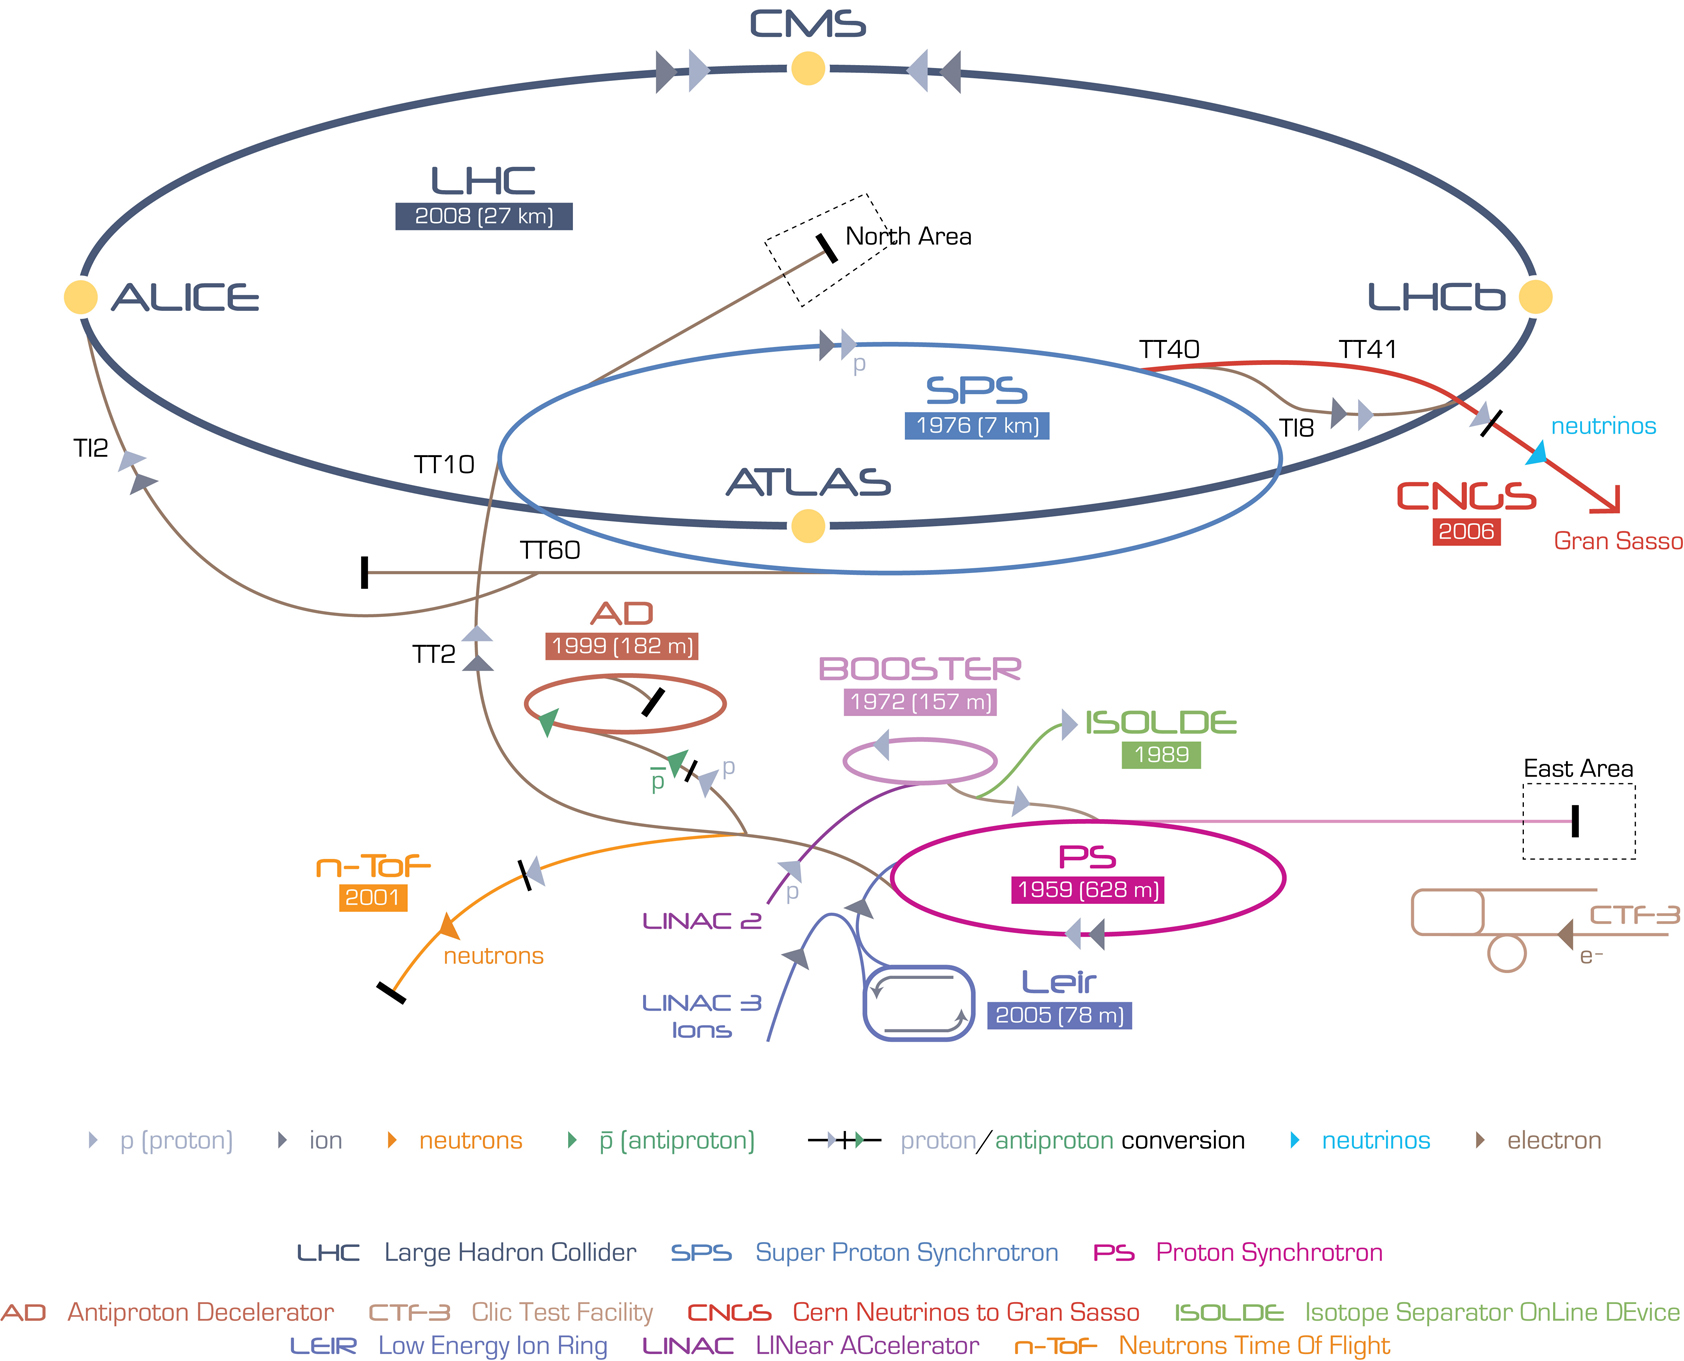
\includegraphics[width=0.6\textwidth]{02_experimental_setup/plots/Cern-Accelerator-Complex.png}
  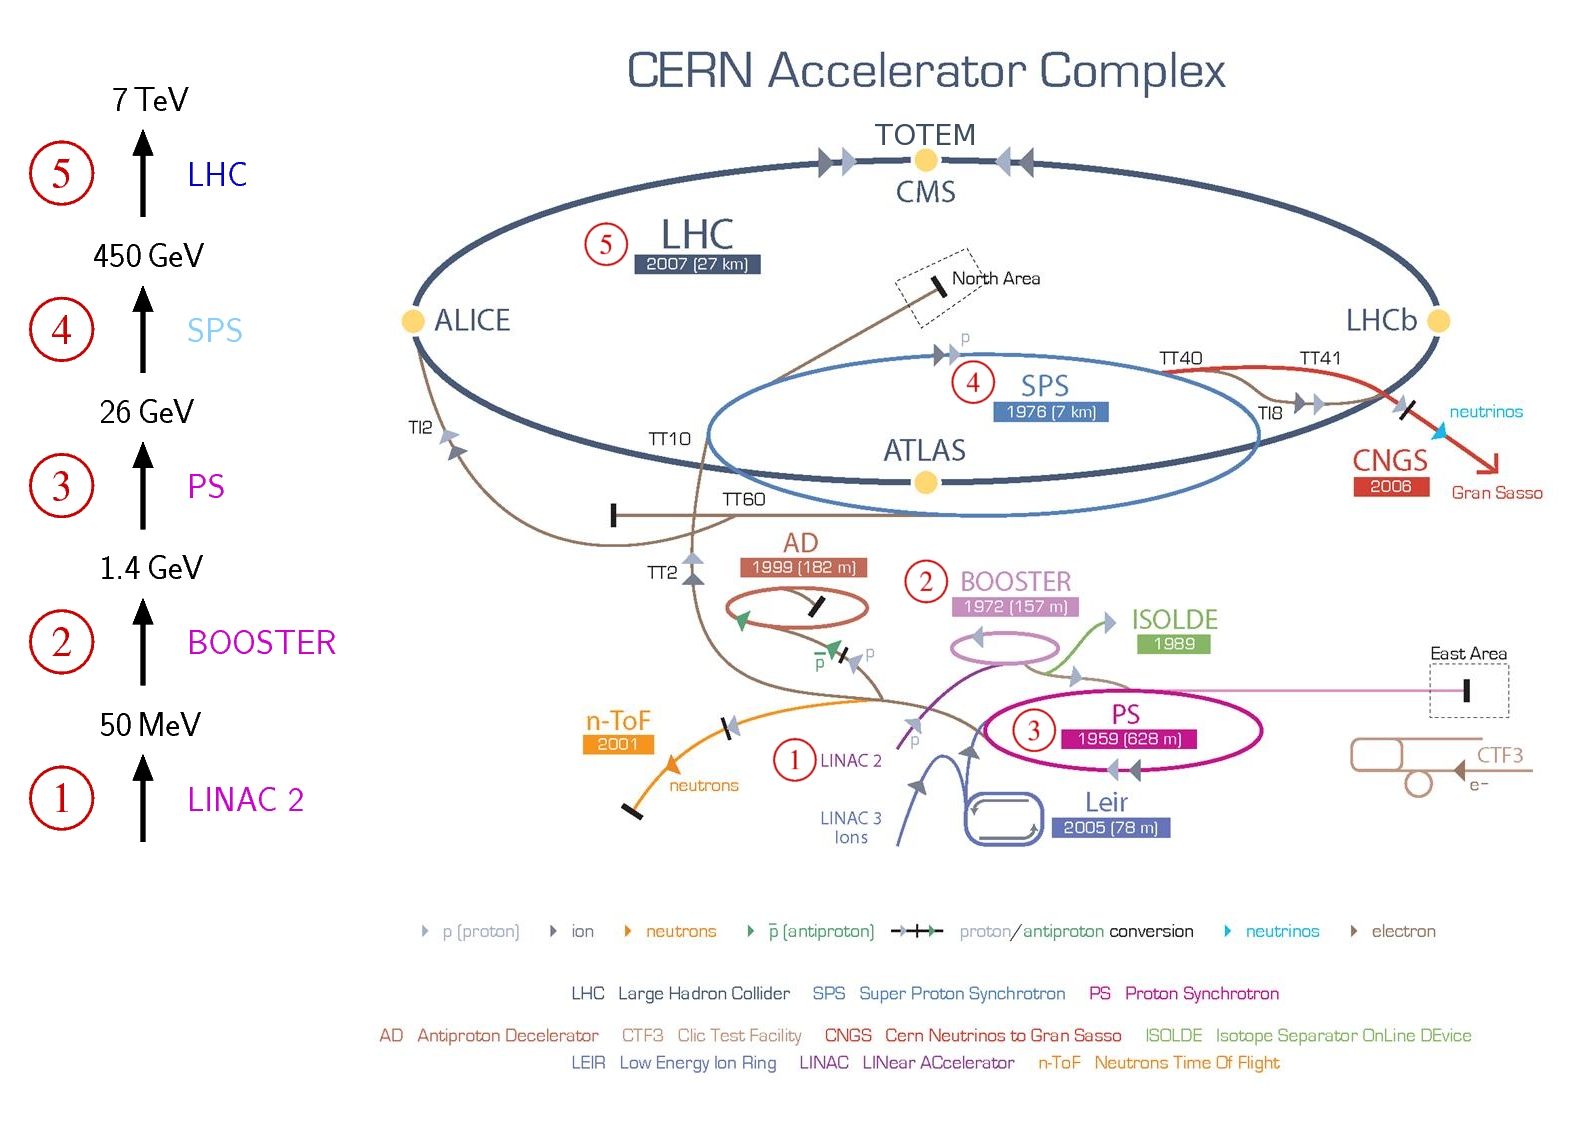
\includegraphics[width=0.8\textwidth]{02_experimental_setup/plots/Cern-Accelerator-Complex-2.png}
  \caption{The complex of accelerators at CERN with their length and particles being accelerated inside.}
  \label{fig:AccelCERN}
\end{figure}

\begin{itemize}
 \item[--] Protons first enter the \textit{Linac2}[?] where they are accelerated up to 50 MeV and sent to Proton Synchrotron Booster (PSB);
 \item[--] \textit{PSB}[?] is composed of four synchrotron rings (to avoid charge repulsion) which raise the energy of the particles to 1.4 GeV
 for injection into the Proton Synchrotron (PS);
 \item[--] \textit{PS}[?] increases the energy up to 26 GeV and takes 3.6 s to get injection to the Super Proton Synchrotron (SPS); 
 \item[--] \textit{SPS}[?] is the second largest accelerator at CERN which comes out with 450 GeV protons injected to LHC.
\end{itemize}

The important accelerator characteristic to perform experimental measurement is the number of coinciding protons 
in coincidence area per time called \textit{instantaneous luminosity} $\mathcal{L}$. The designed value 
at the LHC is $\mathcal{L} = 10^{34}$ cm$^{-2}$ s$^{-1}$. The accelerator was providing $\mathcal{L} = 7.7 \cdot 10^{33}$ cm$^{-2}$ s$^{-1}$
during the run in 2012.

Integral of instantaneous luminosity over the time
is defined as \textit{integrated luminosity} $L$: 
\begin{equation}\label{eq:lumi}
  L  = \int\mathcal{L}dt.
\end{equation}
LHC provided 23.3 fb$^{-1}$ of integrated luminosity for the run in 2012 from which 21.8 fb$^{-1}$ were
recorded by the Compact Muon Solinoid (CMS) detector which is seen from the Fig.\ref{fig:LumiCMS}

\begin{figure}[t]
  \centering
  %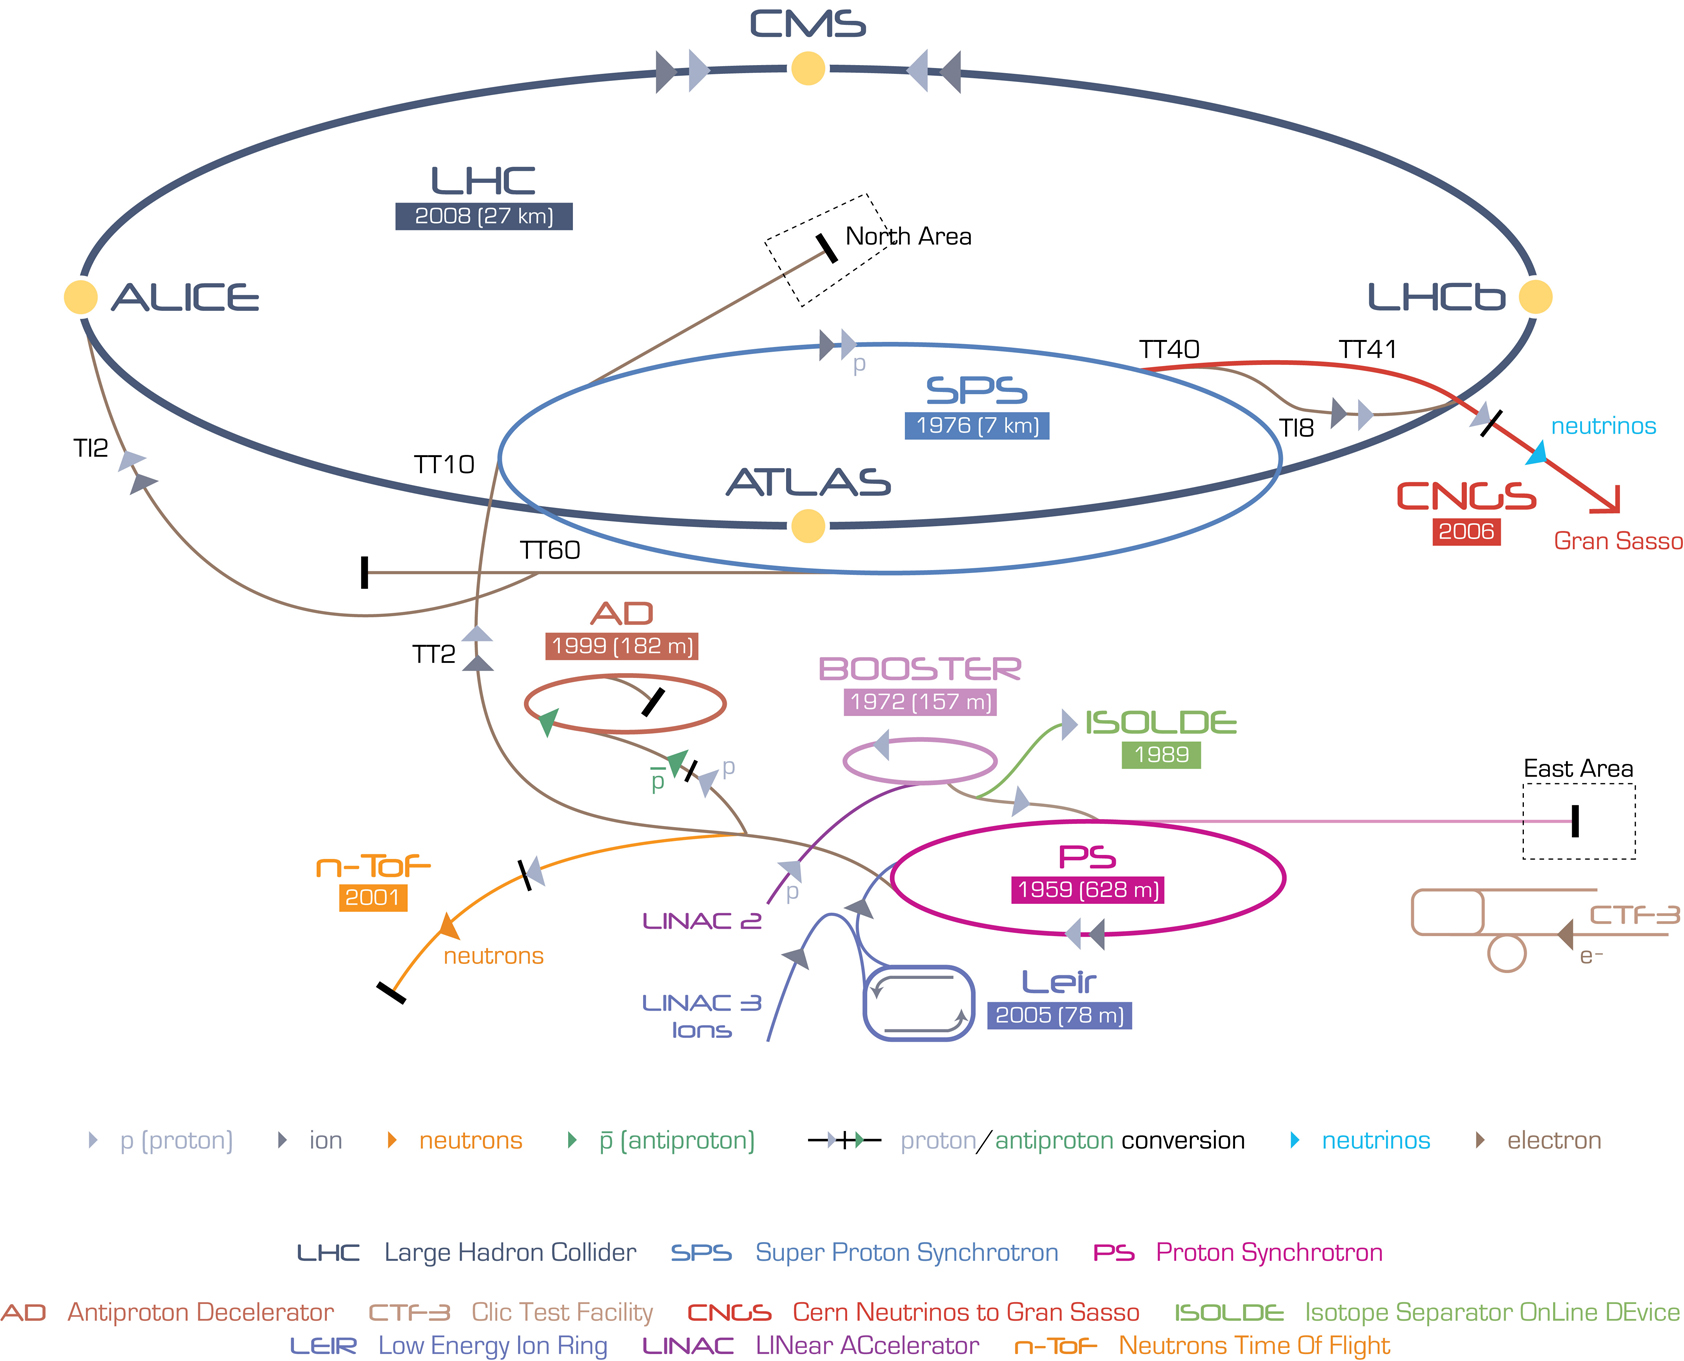
\includegraphics[width=0.6\textwidth]{02_experimental_setup/plots/Cern-Accelerator-Complex.png}
  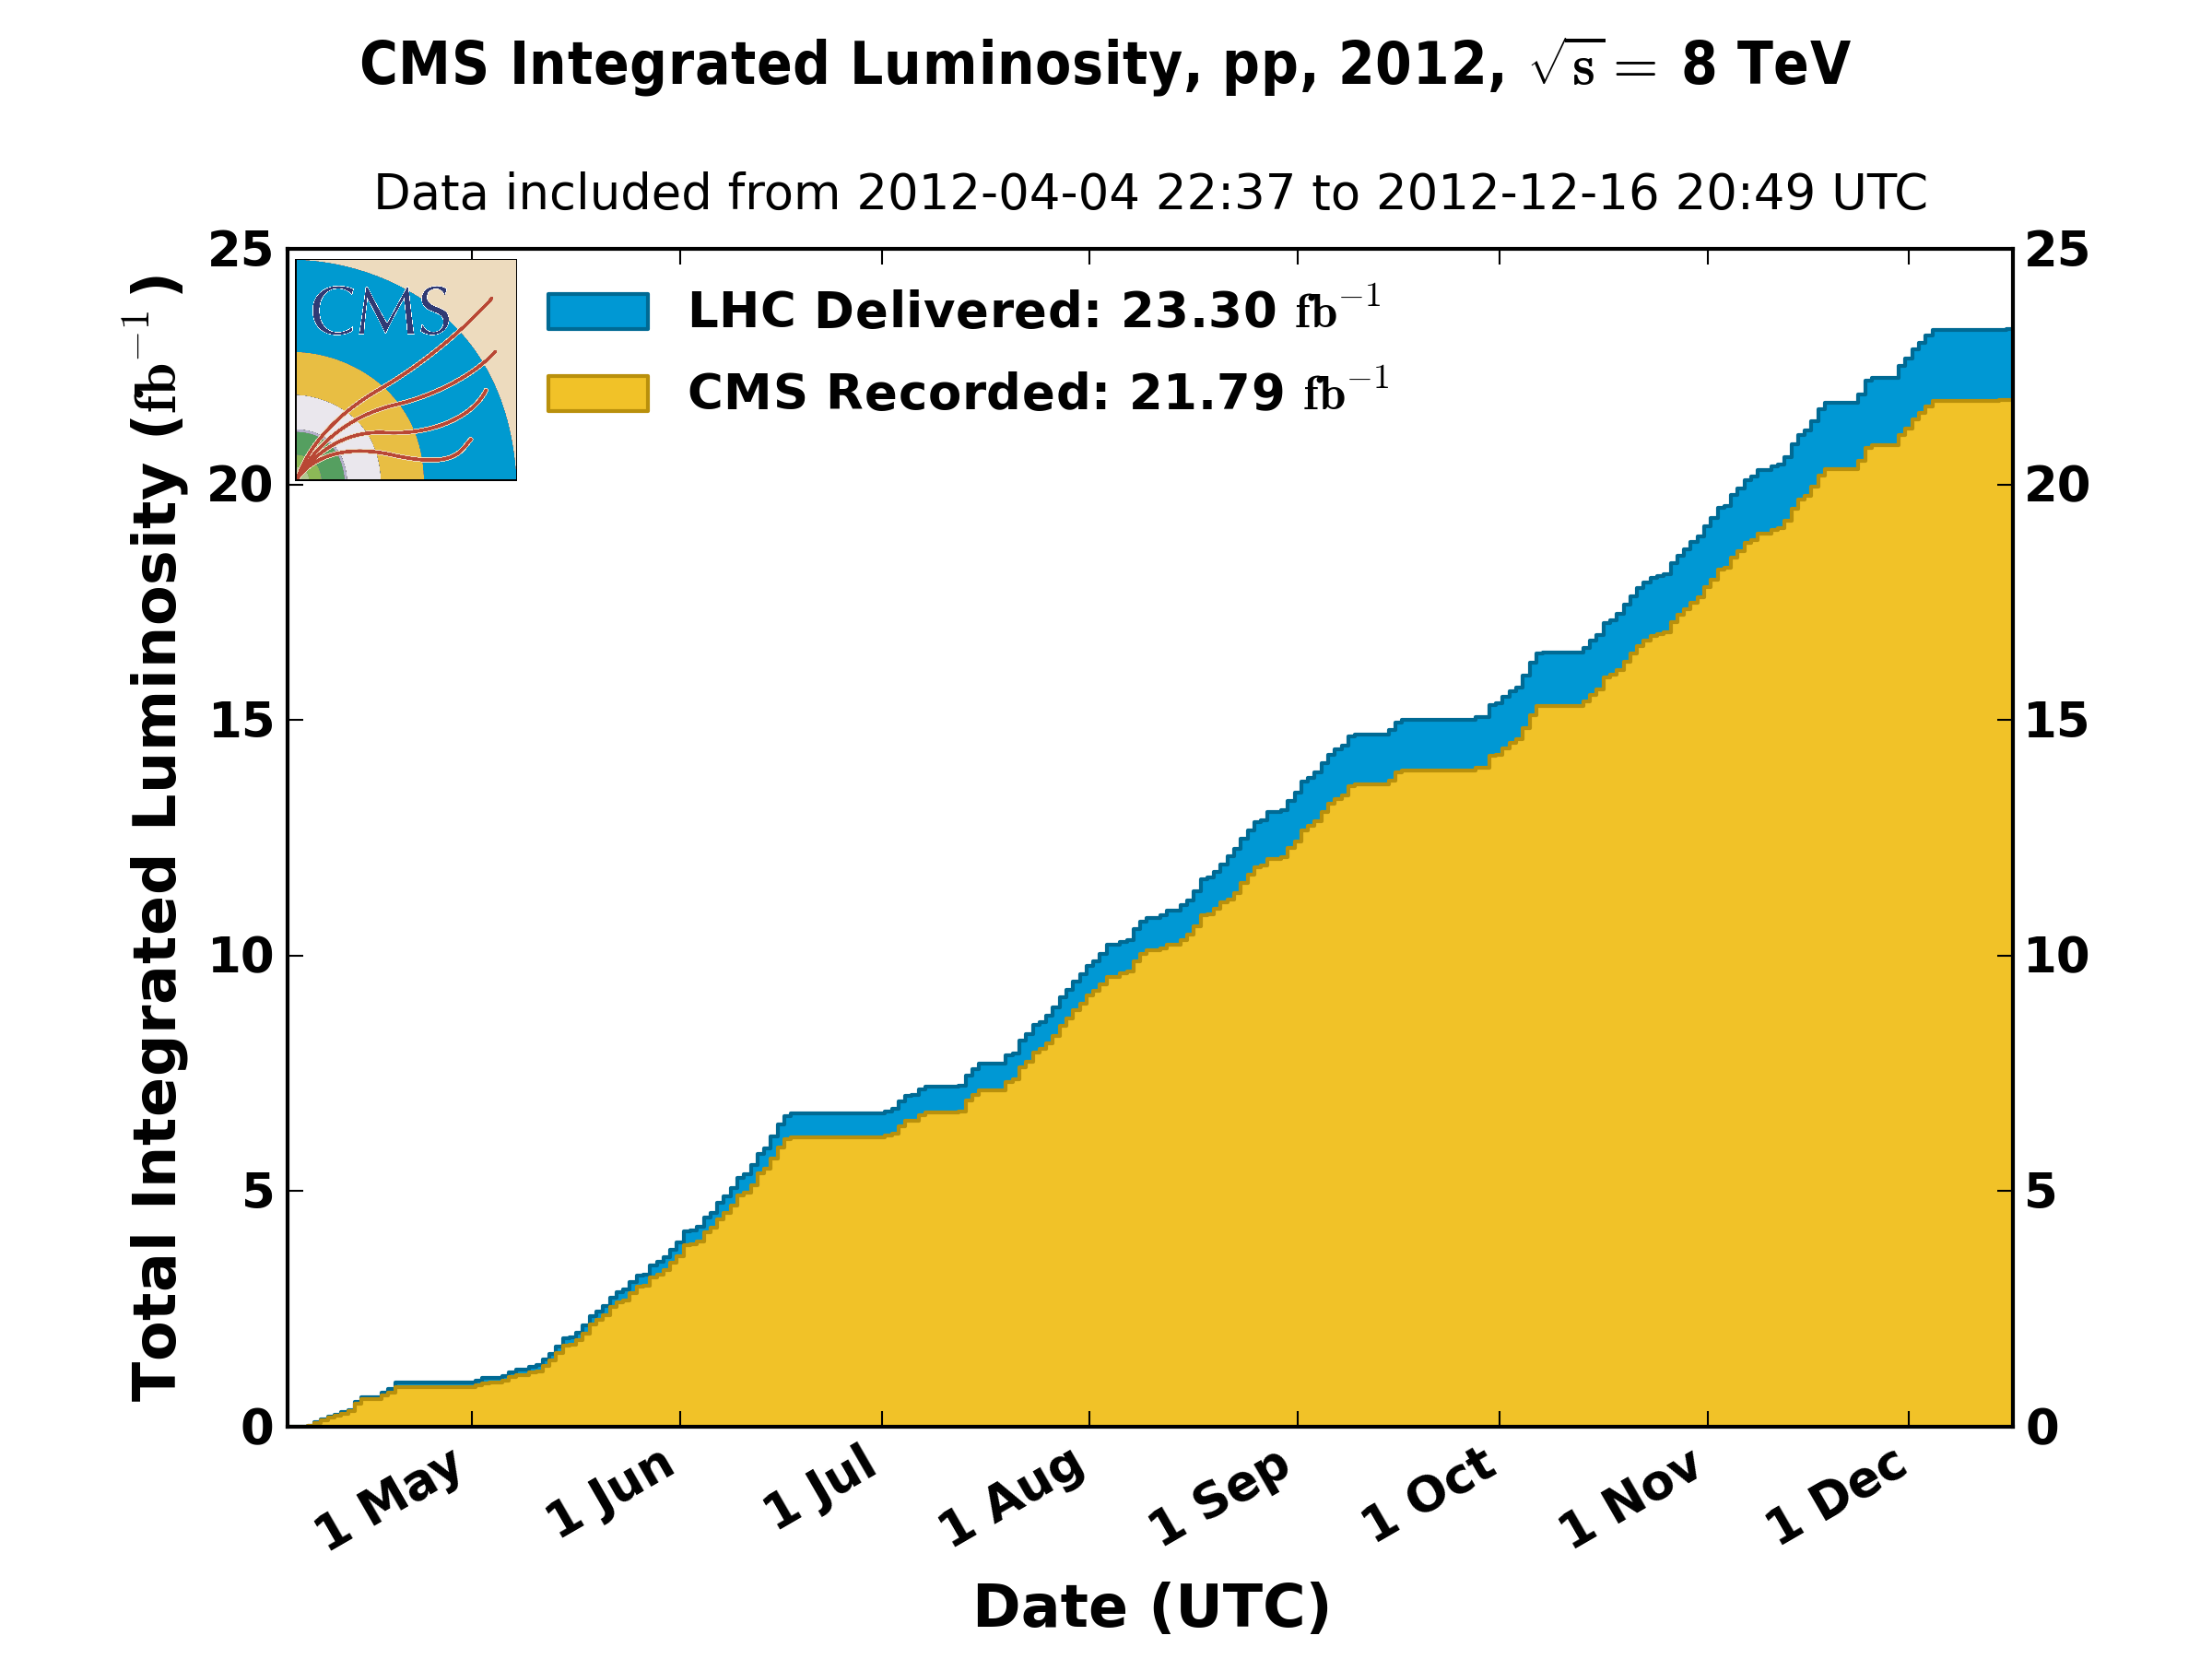
\includegraphics[width=0.6\textwidth]{02_experimental_setup/plots/int_lumi_per_day_cumulative_pp_2012.png}
  \caption{Cumulative luminosity versus day delivered (blue) and recorded by the CMS (orange) for proton-
  proton collisions during stable beam time in 2012.}
  \label{fig:LumiCMS}
\end{figure}

During the 2012 LHC run period $3.16 \cdot 10^16$[?] protons were delivered which means only ~$1$ mm$^3$ of Hydrogen gas 
under the normal conditions is needed (taken the efficiency of proton source to account[?]). 
%http://www.lhc-closer.es/1/3/10/0
%https://indico.cern.ch/event/219327/ -- slide 11

The measurements of collision products are done with the complex particle detectors. There are four of them, 
\textit{ALICE}, \textit{LHCb}, \textit{ATLAS} and \textit{CMS}, on the LHC
ring, each located around the point where beams of particles of different directions are brought together.
These detectors have different construction thus having slightly different goals.

\begin{itemize}
 \item The ALICE (A Large Ion Collider Experiment)\cite{ALICEtdr} is designed to
 work with the heavy ion collisions. The goal of the ALICE experiment studies is
 the strongly interacting matter in extremely high density state called \textit{quark-gluon plasma}. This 
 state of matter provides a unique possibility to find a bare quark without a pair and also to study the early
 Universe which was so dense at the first moments after the Big Bang.
 \\
 The ALICE detector weights 10000 tonnes and is 26 m long, 16 m high and 16 m wide. It sits on the depth of
 56 m below the ground on the territory of France.
 
 \item The LHCb (Large Hadron Collider beauty)\cite{LHCb} is investigating the $CP$ violation and heavy flavour physics via
 the rare $B$ hadron decays. As the $b\bar{b}$ pairs are mostly produced in the forward and backward directions, 
 and their production cross section is very high there was no need to construct a big and expensive $4\pi$ detector 
 complex. For this reason the LHCb is a one side spectrometer corresponding to the forward beam direction.
 For a better detection of the $b$-decays the LHCb features a movable tracking system which can go very close
 to the beam pipe.
 \\
 The LHCb detector weights 5600 tonnes and is 21 m long, 10 m high and 13 m wide. It sits on the depth of 100 m 
 below the ground on the territory of France.
 
 \item The ATLAS (A Toroidal LHC ApparatuS)\cite{ATLAS} is one of the two general purpose detectors on the LHC. It has many physical
 goals -- from Standard Model examination and Higgs searches to the studies of dark matter, extra dimensions and new physics.
 These tasks are mainly similar to the ones from the CMS experiment (the second general purpose detector on the LHC ring), but
 it uses different technical solutions.
 \\
 The ATLAS machine is built around the beam pipe such that the collision point is located in its center. It consists of the 
 inner tracking system and calorimeter, both surrounded by the barrel (2 T) and toroid magnets (0.5 to 1 T). The muon spectrometer
 is located on the outer layers of the detector.
 \\
 Having a length of 45 m, a height of 25 m and a width of 25 m ATLAS is a largest particle detector complex in the world. While the mass 
 of it is rather low reaching 7000 tonnes. It sits in a cavern 100 m under the ground on the territory of Switzerland.
 
 \item The CMS (Compact Muon Solenoid) is the second general purpose detector on the LHC. A more detailed description of this apparatus will follow in the
 section \ref{sec:CMS}.
 
\end{itemize}


Two much smaller experiments are also located at the LHC ring alongside the four larger ones mentioned above. They are focused on forward particles
researches which do not collide but rather brush past each other and continue their flow along the beam direction. Thus these facilities do not
need to be based around the beam coincidence points. The names of the two experiments are \textit{LHCf} and \textit{TOTEM}.

\section{The Compact Muon Solenoid}\label{sec:CMS}

The analysis presented in this work was performed on the data recorded by the Compact Muon Solenoid (CMS) detector\cite{CMSatLHC} during the 2012
run period in proton-proton collisions with center-of-mass energy $\sqrt{s} = $8 TeV. This section will describe in more detail 
the construction and performance of the CMS machine.

Any particle detector is being constructed with respect to the measurements which are planned to be done on it. Different physical
tasks provide special requirements for specific experimental setup parts. If the plan is to measure Standard Model decays
($W$, $H$, $Z'$ decays with leptons in final state), the detector complex has to comprise a precise electromagnetic calorimetry and 
muon systems for a better lepton reconstruction. To measure the QCD processes with jets in final states, a
good hadronic calorimetry has to provide absolute energy determination with fine resolution. To look for heavy resonances one needs a
precise detection in the central region, perpendicular to the beam direction. Unlike for the low mass particles, where the tracking
has to cover the forward regions. The parts of the detector located in the direction of beam flow are also important to measure the 
total transverse missing energy. A particle identification precision and muon detection relies much on a magnet system which bands the charged 
particles differently corresponding to their energy and charge. This also makes it important to choose the optimal magnet
shape and power. To gain precise $b$- and $\tau$ identification, good inner silicon
pixel and strip detectors have to be operated. Also taken into account the designed luminosities (see Sec.\ref{sec:LHC}) and bunch spacing of 25 ns at the LHC,
the detectors have to deal with multiple interactions per collision - pile up. Not to get distorted by a large amount of particles 
flowing to one sensor unit, the detector must have a fine enough granularity and radiation hardness.
And in the end the price and feasibility play a crucial role in the detector complex creation.

The CMS facility being a general purpose detector was designed to make it's parts fulfill as many physical goals as possible.
The final onion-like construction of the machine is shown on the Fig. \ref{fig:CMSview}. The overall detector size reaches 28.7 m in length
and 15.0 m in width. The total weight of the facility is 14000 tones, which makes the CMS the heaviest particle detector on the
LHC. The detector is cylindrically symmetric around the beam pipe and also symmetric to left and right sight along the beam direction
relative to the collision point.

\begin{figure}[t]
  \centering
  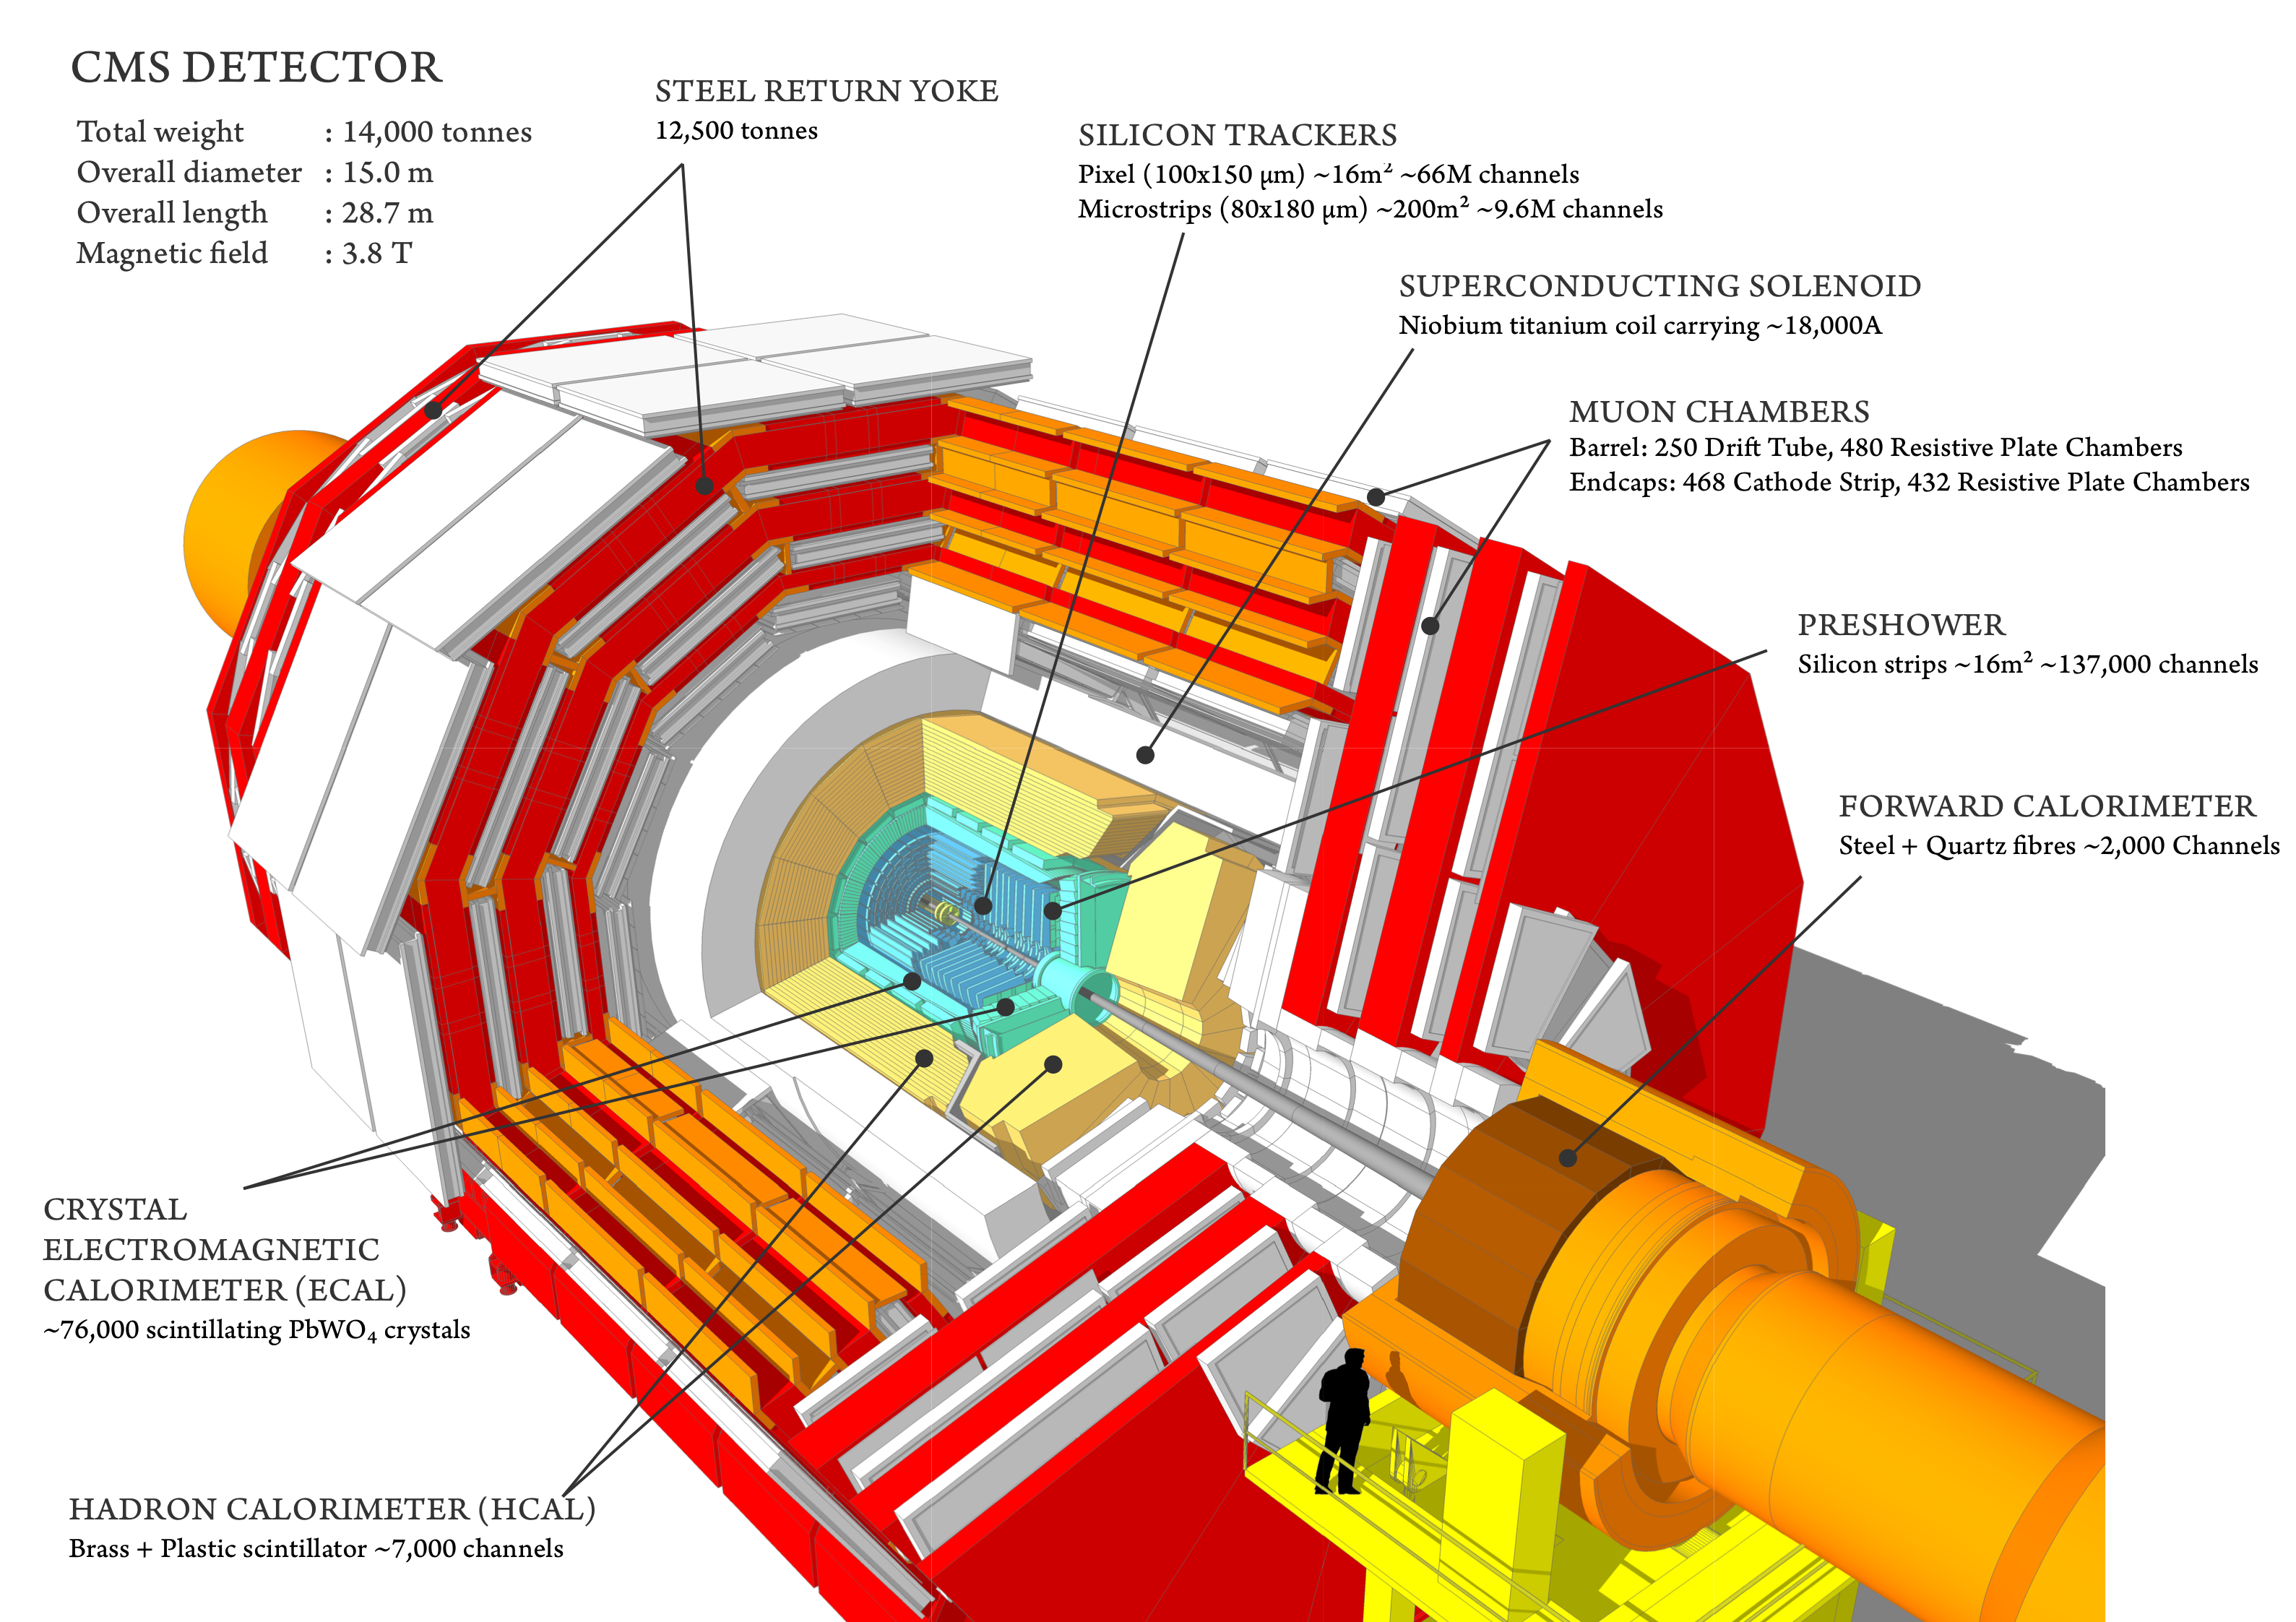
\includegraphics[width=0.8\textwidth]{02_experimental_setup/plots/cms_120918_03.png}
  \caption{Sectional view of the CMS detector. The LHC beams collide in the center of the 
  machine. The central axis of the detector corresponds to the beam direction. Position of different
  components is highlighted.}
  \label{fig:CMSview}
\end{figure}

The common coordinate system is important for measurement consistency. For the CMS experiment the origin  
is assumed to be located at the nominal collision point, the $x$-axis is pointing to the center of the 
LHC ring and the $y$-axis is pointing vertically upwards. Thus the $z$-axis points along the beam axis towards the
Jura mountains. As the detector is symmetric around the beam pipe, it may be convenient to use cylindrical or spherical
coordinate systems. The azimuthal angle $\phi$ is measured from the $x$-axis in $(x-y)$ plane and the polar angle $\theta$ --
from the $+z$-axis. The radial coordinate $r$ is a distance from the beam pipe. Often the variable \textit{pseudorapidity}
$\eta$ is used instead of the polar angle:

\begin{equation}\label{eq:eta}
  \eta = -\ln(\tan(\frac{\theta}{2})) = \frac{1}{2}\ln\frac{|\bar{p}| + p_{L}}{|\bar{p}| - p_{L}},
\end{equation}
where $\bar{p}$ is the particle momentum vector and $p_{L}$ is it's projection on the $z$-axis, or longitudinal component.
The other variable which can be used instead of $\eta$ for the massive particles is the \textit{rapidity} $y$:

\begin{equation}\label{eq:y}
  \eta = \frac{1}{2}\ln\frac{E + p_{L}}{E - p_{L}},
\end{equation} 
where $E$ is the energy of the particle.

The momentum and energy transverse to the beam direction, denoted as $p_{T}$ and $E_T$, are also commonly used in the data analysis. 
They are defined in the $(x-y)$ plane. Another variable is responsible for the energy imbalance in transverse plane is a
\textit{missing transverse energy} $E_{T}^{miss}$.

\subsection{Solenoid magnet}

The CMS detector features a 4T superconducting solenoid 13 m in length and 6 m in diameter shown on the Fig.\ref{fig:solenoid}. 
The flux is returned through a 10000 tonnes yoke \cite{CMSatLHC}. Historically the main stress of the CMS detector was 
addressed on the construction of a precise moun detection system, as at the time when the facility was designed, there 
were no silicon pixel tracker technologies providing material with sufficient radiation hardness and readout speed. Thus, 
the tracking could have had a bad performance. So a good muon identification would
rescue some physics processes reconstruction. A strong magnetic field plays a very important role for identifying high energetic
particles as muons, bending them enough on their pass to the muon system.

\begin{figure}[t]
  \centering
  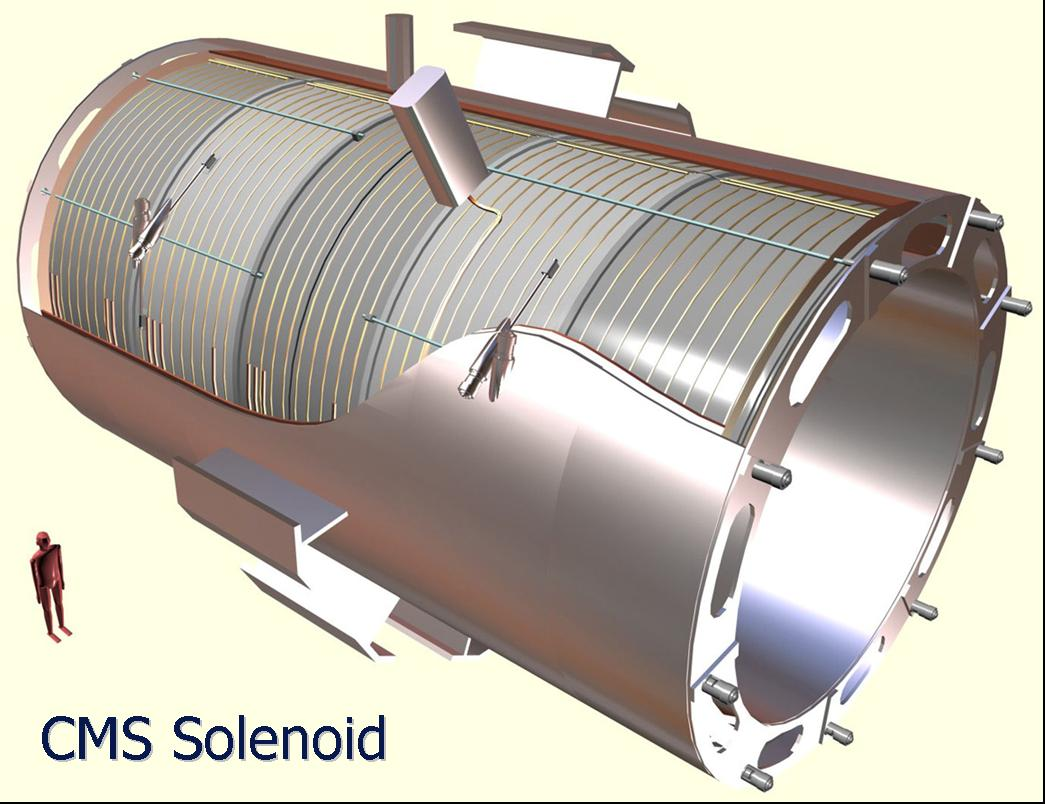
\includegraphics[width=0.6\textwidth]{02_experimental_setup/plots/CERN_CMS_Solenoid_schematic.png}
  \caption{The schematic view on the CMS solenoid}
  \label{fig:solenoid}
\end{figure}

The strength of the magnetic field sets the limit of the size of tracking and calorimetry systems. Most of the tracks should reach the 
calorimeter before they start to band back to the beam direction. The solenoid magnet geometry limits the tracking precision to
the central pseudorapidity ranges, as the forward regions will have unbanded tracks which are not influenced by a magnetic field.

\subsection{Tracking Detector}
% \subsection{Electromagnetic Calorimeter}
% \subsection{Hadronic Calorimeter}
% \subsection{Muon Detector}
% \subsection{Trigger system}
% 
% \section{Upgrade for RunII}
% \subsection{CMS Pixel Tracker Upgrade}